
As briefly mentioned in the Introduction chapter, our goal is to utilize Leap Motion controllers combined with the pre-trained ANN model. In the following chapter, we will explore datasets used for our training and the obstacles that came along with them. Then we will discuss the model training itself and its results. At last, we will deploy the trained model for real-time recognition in a C++ environment.


\section{Dataset Description}

Among many publicly available datasets for gesture recognition are only a few containing necessary skeletal information similar to those yield by Leap Motion controllers. We have selected ASL Dataset and SHREC 2017 Dataset created in conjunction with \cite{avola} and \cite{shrec} respectively, often used as benchmark measurement for trained model accuracy.

\subsection{SHREC 2017 Dataset}

The SHREC dataset contains sequences of 14 dynamic hand gestures. Each gesture was performed between 1 and 10 times by 28 participants in two ways, using one finger and the whole hand. All participants were right-handed. The length of sample gestures varies between 20 to 170 frames, making some samples too short. The variation of frames makes it too incosistent for our usage in real-time deployment and for such unsuitable.

\subsection{ASL Dataset}

ASL Dataset consists of 30 hand gestures, 18 static gestures, and 12 dynamic gestures. Gestures were collected from 20 different people. 13 were used to form the training set, while the remaining 7 formed a test set. Each person performed 30 hand gestures twice, once for each hand, and each gesture is composed of fixed 200 frames as oppose to frame varying SHREC dataset \cite{avola}. 

After further inspection of the ASL dataset, we have discovered possible mislabeling of features. Specifically, taking a look at internal angles of gesture for number 1, we can see that 1 requires the ring finger to straighten out instead of the index finger. The same can be said about the gesture of number 2, where it appears to have the ring finger and middle finger straight out instead of the index finger and middle finger. It is unclear whether there are other mislabeling among the features. The mislabeling in itself is not an obstacle for training because the features are independent of each other, and the ANN can still learn on them, but the issue will arise in real-time classification, where raw data must be preprocessed identically as the training data. We decided not to use ASL Dataset for our purposes but only to benchmark model architecture.


\subsection{Handicrafted Dataset}
\label{handicrafted_dataset}
By not using ASL Dataset we have lost a set of static gestures. Also, we want to have the ability to provide the training with our own sets of gestures and not to be bound only to those publicly available. For such purposes, we had created a simple interactive data sampler in the form of a console application.

The sampler saves each sample in .txt format, one line by timestep $T$, frame yield by LMC, each line containing a set of features. Features were selected and computed as previously described in section \ref{sec:feature_extraction}. The order of features in a line $x_t$, at time $t$ is as follows.


\begin{equation}
	{x_t = \{\omega_0, ...,\omega_4, \beta_0, ..., \beta_4, u_0,v_0,z_0, ..., u_5,v_5,z_5, \gamma_1, \gamma_2, \gamma_3\}}
\end{equation}

All samples contain the same number of timesteps, specified at the beginning by the user or using default value of $T=60$. The number of timesteps should be further analyzed inorder to find the optimal value. The value of timestep mostly affects the delay rate between presented gesture and its prediction in a real time environment, higher creates greater delay. Also, if the value is too high the dynamic gesture may have minimal role in the sample and we won't get desired behavior from our ANN. If the number is too low, the dynamic gesture may not be captured completely and the rate of performed predictions increases, creates greater demand on hardware. 

The recording is initiated by key command, but the data collection does not start until the user's hand is in LMC's field of view. Data collection stops once the set of collected frames $\Theta$ matches $T$, or if the hand falls out of LMC's view. Features of missing timesteps are then set as zeroes. The sampling can be subdivided into 3 types:

\begin{enumerate}
	\item \textbf{Single recording} records and saves a single sample. The next recording must be initiated by the user.
    \item \textbf{Open recording} records and saves samples continuously. We recommend using the method only for static gestures. It is best to have a full control over recording a dynamic gesture, its beginning, and its end, along with its most significant sequence.
    \item \textbf{Recording significant frames} records and saves a single sample. The next recording must be initiated by the user. The number of collected frames $\Theta^*$ is greater than the required number of timesteps $|\Theta^*| > T$. The last frame is excluded if $|\Theta^*|$ is not even. We will then calculate a \textit{significance} between $x_t$ and $x_{t+1}$.
    The \textit{significance} of an interval is calculated as average euclidean distances of palm and finger tip positions $P$ between $x_t$ and $x_{t+1}$.

    \begin{equation}
        {s_{(t, t+1)} = d(P_{t}, P_{t+1})}
    \end{equation}

    \begin{equation}
        {S = \{s_{(0, 1)}, ...,s_{(t, t+1)}\}}
    \end{equation}

    Frames are then selected into $\Theta$ by most significant to least significant till $|\Theta| = T$. The following cases must be considered:
    \begin{itemize}
        \item $|\Theta| + 2 \leq T \land x_t$ and $x_{t+1} \notin \Theta$, both frames $x_t$ and $x_{t+1}$ will be added to $\Theta$.
        \item $|\Theta| + 1 = T \land x_t$ and $x_{t+1} \notin \Theta$, both $x_t$ and $x_{t+1}$ are possible candidates for $\Theta$ but only one can be added due to the size $|\Theta|$ which would reach the limit after addition of one. In order to decide which to pick we will compare the significance $s_{(t-1, t)}$ and $s_{(t+1, t+2)}$, and pick greater of the two.
        
        It is possible that $x_t$ is the first frame of $\Theta^*$, in which case we will pick $x_{t+1}$ to be included in $\Theta$. On the other hand, if $x_{t+1}$ is the last frame of $\Theta^*$, we will pick $x_t$.
        
        \item $x_{t} \notin \Theta \land x_{t+1} \in \Theta$, frame $x_t$ is picked
        \item $x_{t} \in \Theta \land x_{t+1} \notin \Theta$, frame $x_{t+1}$ is picked
    \end{itemize}
    
    The method is recommended for sampling dynamic gestures. We attempt to capture the most important part of a dynamic gesture, its movement. 

    The most challenging part of creating a dataset is when we do the sampling itself. We want to keep in mind the variety of samples, meaning angles, positions and additionaly when it comes to dynamic gestures, various speeds and starting positions. Also, the factor of overlapping characteristics of gestures must be taken into considiration. For example an open hand and open handed swipe right may share some similar sequence of frames. Despite introducing sampling specifically for dynamic gestures, it can still be difficult to create a diverse enough dataset, which still holds key properties of the gesture and will enforce the model to learn on its characteristics.

    For our purposes we created a dataset, which consists of 7 static gestures (fist, 1-pointing, 2-peace sign, 3, 4, 5-open fist, pinch) and 2 dynamic gestures(swipe left, swipe right), each of average 370 samples performed by both hands. 

\end{enumerate}


\section{Model Training}
\label{sec:model_training}

We selected Python to be our primary language for training the ANN mode along with the web-based interactive development environment Jupyter Notebook. One of the main reasons to pick Python over other available languages was its wide range of libraries and scientific packages supporting machine learning tasks. Most importantly, Keras, a high-level deep learning API integrated with TensorFlow, enabling the user to create and train model structures in very few steps.

SHREC Dataset and ASL Dataset were used to benchmark the model. For the purpose of real-time recognition, we trained the model on our handicrafted dataset consisting of numbers between 1 to 5 and simple dynamic gestures swipe left and right, where each gesture had 150 to 600 samples, 90 frames per sample, recorded in various angles, positions and speeds. 

Each dataset was then split into 80\% for the training set and 20\% for the testing set, where 10\% of the training set was used for validation. Each feature was then normalized via min-max scaler formula:

\begin{equation}
    { x' = \frac{x - Min(X)}{Max(X)-Min(X)}\;\;\; x \in X}
\end{equation}

\subsection{DLSTM architecture}

At first, we followed the proposed architecture of 4 layers stacked LSTM by Avola D., Bernardi M. et al. \cite{avola}. We trained the model using 800 epochs and 0.0001 learning rate, which were proved to be optimal hyperparameters as described in section \ref{sec:dlstm_params}

Benchmarking the model on ASL Dataset resulted in similar accuracies as in \cite{avola}. Our handicrafted dataset had also achieved high results.

Despite achieving high accuracies on ASL dataset and our original dataset, the model itself did not perform well in a real-time environment. More specifically, the 4 layered LSTM architecture struggled with dynamic gestures. The model did not learn the gesture in relation to the movement but rather on its most occurring position in the recorded sequence, which in the case of swipe right was the palm's final position. The model successfully classified test samples because all gestures swipe right contained some frames where the palm position was on the right. Once we presented the model in a real-time environment with an open palm on the right, without the swipe movement, it classifies such gesture as swipe right, which is an undesired behavior. 

It is unclear whether the model would perform better with more stacked LSTM layers or not. Other possibility would be insufficent dataset, but we were able to utilize the same dataset on different architecture in real-time environment. Hence we concluded that the DLSTM architecture was not suitable for our purposes.

\subsection{Two-Layered Bidirectional LSTM architecture}

After an unsuccessful attempt to utilize DLSTM, we turned over to two-layered bidirectional LSTM architecture proposed in \cite{bidirect_dynam}. The proposed architecture was meant and trained on dynamic gestures only, not knowing how it will perform on static gestures. On the other hand, static gestures can be treated as a special type of dynamic gesture, having one frame stretched out to the desired number of timesteps. Not to mention our dataset was constructed in a way where static gestures have a slight difference in coordinates between $t$ and $t+1$, making it possible to look at the static gesture as a very slow type of dynamic gesture.

\subsubsection{Selection of the Optimal Dropout Rate}

To avoid the problem of overfitting, we used dropout regularization. 
A technique that, during training, randomly drops out a number of neurons in layers, thus ignoring their connections in the network. This creates a new smaller network and, in essence, simulates model ensembling without creating multiple networks.

We used ASL Dataset for its variety in samples and possible more complexity over our own handicrafted dataset. Despite its mislabeling of features, it still serves well for model benchmarking and validation.

The optimal dropout rate was selected through several experiments using dropout values in a range of 0.0 to 0.9. As seen below, not using dropout regulation caused a visible difference between train and validation accuracies through the course of training. The difference stayed poor, almost the same up to the value of 0.4, which showed improved results but not necessarily optimal. The difference was most promising when using dropout values of 0.5 and 0.6, where 0.6 performed better. However, the performance gets worse from 0.7 and on. The overall results indicate that the optimal dropout value is between 0.5 and 0.6. The value of 0.6 is satisfactory enough for our uses.

\begin{figure}[h]
	\centering
    \subfloat[\centering No dropout regularisation applied]{{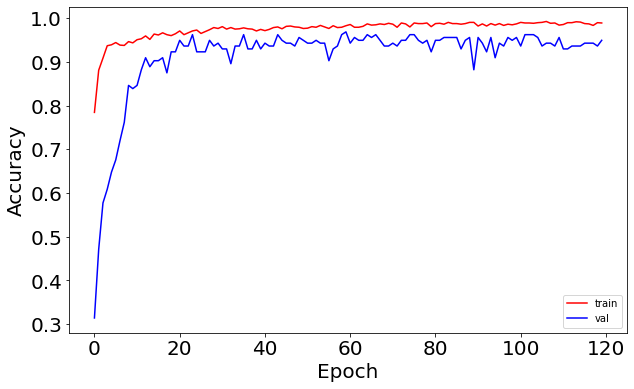
\includegraphics[width=6cm]{dropout_0.png}}}%
    \qquad
    \subfloat[\centering Dropout rate = $0.6$]{{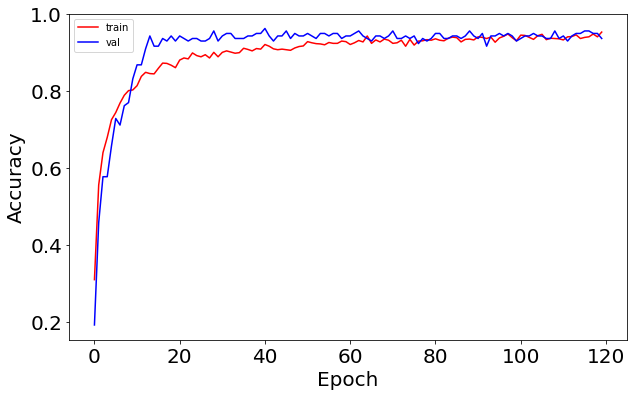
\includegraphics[width=6cm]{dropout_6.png}}}%
    \caption{Train accuracies compared to validation accuracies through the course of learning}
\end{figure}

\subsubsection{Optimal number of stacked layers}

While searching for optimal dropout rate, we had performed the experiment across different depths of the network, more precisely 1 to 5 layered bidirectional LSTM networks. The dropout value appeared to have held the same characteristics for the different number of stacked layers.

The additional testing of the network's depth was to find out whether using a different number of layers than proposed in \cite{bidirect_dynam} would make any improvements in overall prediction performance.

To find the optimal depth of the network, we have adopted $k$-fold Cross-validation. Cross-validation is often used to evaluate the performance of machine learning models on limited datasets. The entire data set is split randomly into $k$ folds, in our case $k=5$, then train the model using $k-1$ folds and hold the remaining fold to measure the model's accuracy. We will be repeating this process for each fold and then calculate the average performance across all folds.

\begin{table}[ht]
    \centering
    \caption{Average recognition accuracies across different depths of bidirectional lstm architectures using 5-fold on 200 epochs}
    \begin{tabular}{ | p{4.5cm}| p{4.5cm} |} 
        \hline
        \hfil \textit{Number of layers}
        & \hfil \textit{5-fold (\%)}\\
        \hline\hline
        \hfil 1 				& \hfil 88,14			\\
        \hline
        \hfil 2 				& \hfil 89,07		\\
        \hline
        \hfil 3 				& \hfil 87,48		\\
        \hline
        \hfil 4 				& \hfil 86,31		\\
        \hline
        \hfil 5 				& \hfil 87,98		\\
        \hline
    \end{tabular}
    \label{tab:HT_results_table}
\end{table}

The two-layered bidirectional LSTM architecture acquired the best performance results compared to other depths. Increasing the number of epochs would improve the results of architectures with more layers, but we would suffer on the side of the training time required. In conclusion, choosing the two-layered architecture is a good compromise between accuracy and training time.

The two-layered bidirectional LSTM architecture was successful in learning dynamic gestures base on its characteristic movement and it was also successful in classifying static gestures, both in real-time recognition.

\section{Real-time recognition}
\label{real_time_recognition}

The demo application for real-time recognition is in the form of a simple console application, supporting multiple LMCs using MultiLeap \cite{tomasMultileap} library described in chapter \ref{ch:multileap} and with key commands for LMC calibration. When a hand gesture is presented, the application prints out the prediction, which is considered a valid prediction if the value passes the threshold of 90\% accuracy. The demo application served mainly for debugging and experimental purposes.

For real-time recognition, we chose C++ as our primary language since C++ and C\# are widely used programming languages in graphic engines such as Unity, PhyreEngine, or Unreal, which opens the possibility of integrating our application into graphic engines in future works.

\subsection{Cppflow 2}

Our application uses the trained model from section \ref{sec:model_training} and deploys it in C++ environment. More specifically, we exported the model in .tf file format and imported it into C++ using CppFlow 2.

Cppflow 2 is an API created by Sergio Izquierdo, allowing the user to run TensorFlow in C++ without the necessity of installing and compiling TensorFlow itself. CppFlow 2 serves as a Tensorflow C API wrapper providing a simple C++ interface similar to TensorFlow callings in Python environment \cite{cppflow}. 

\subsection{Sliding window}

The data collection, frame collection yield by LMC, starts once a hand is presented in LMC's field of view and stops if the hand falls out of the view. Let us introduce a situation where during the stream of data yield by LMC, we change our hand gesture from a "fist" to a "peace sign". We want to classify both of these gestures, but how do we determine where one gesture ends and the other starts. To tackle the presented scenario, we adopted the concept of \textit{sliding window}.

The basic idea is to have a window of fixed size $T$, which slides through our data stream and captures a certain portion of it. It is important to remain the same $T$ value as we chose to record our dataset. Otherwise, the shape of the captured data would differ from the input shape of our trained model. It is worth mentioning that using a wider window size creates a noticeable time delay between a presented gesture and its prediction. On the other hand, using a size too small, there would be a possibility of not capturing a dynamic gesture completely, leading to possible inaccurate predictions. In our case we used $T = 60$. Considering a situation where a collected data is less than $T$, the missing data are then set to zeroes. If we present more than one hand, the stream is invalidated, collected data are flushed, and the window will begin its sliding again once there is only one hand in the controller's view.

\begin{figure}[ht]
	\centering
    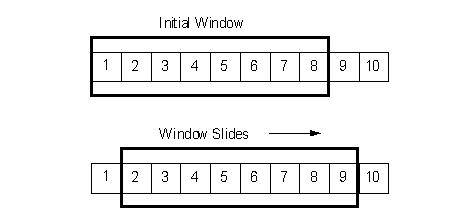
\includegraphics[width=8cm]{sliding_window.png}
	\caption{General idea of a sliding \cite{sliding_window_img}}
	\label{fig:sliding_window}
\end{figure}

For each window, we then calculate features for classification and output the prediction of the captured portion. Features must be preprocessed exactly the same as they were for model training, in our case, same as described in section \ref{sec:feature_extraction}. 

The window slides by 10 frame, in other words throws away oldest frames and adds in newest acquired. The slide rate should be further tunned for optimal value. If we throw away too many frames, we risk of leaving some gestures unclassified. On the other hand, sliding by one frame can be demanding on hardware, where weaker computer builds may not be able to keep up and the prediction may stutter.

